\section{PROCEDIMENTOS METODOLÓGICOS}\label{sec:metodologia}

O \emph{pipeline} de processamento desta pesquisa (Figura~\ref{fig:pipeline}) foi desenhado para garantir reprodutibilidade estrita. Cada etapa registra um identificador de versão do código, os parâmetros utilizados e o resumo criptográfico (\emph{hash}) dos dados de entrada. Dessa forma, todos os resultados podem ser regerados deterministicamente a partir dos artefatos salvos. O código-fonte integral desenvolvido para este estudo está disponível publicamente no repositório GitHub: \url{https://github.com/gabrielfmcoelho/Modelagem-de-tipos-de-processo-e-de-caminhos-tipicos-a-partir-de-registros-de-atividades}.

\begin{figure}[htbp]
\centering
\caption{Etapas do \emph{pipeline} de processamento, da extração no \emph{data lake} ao catálogo de tipos de processo e caminhos típicos.}
\label{fig:pipeline}
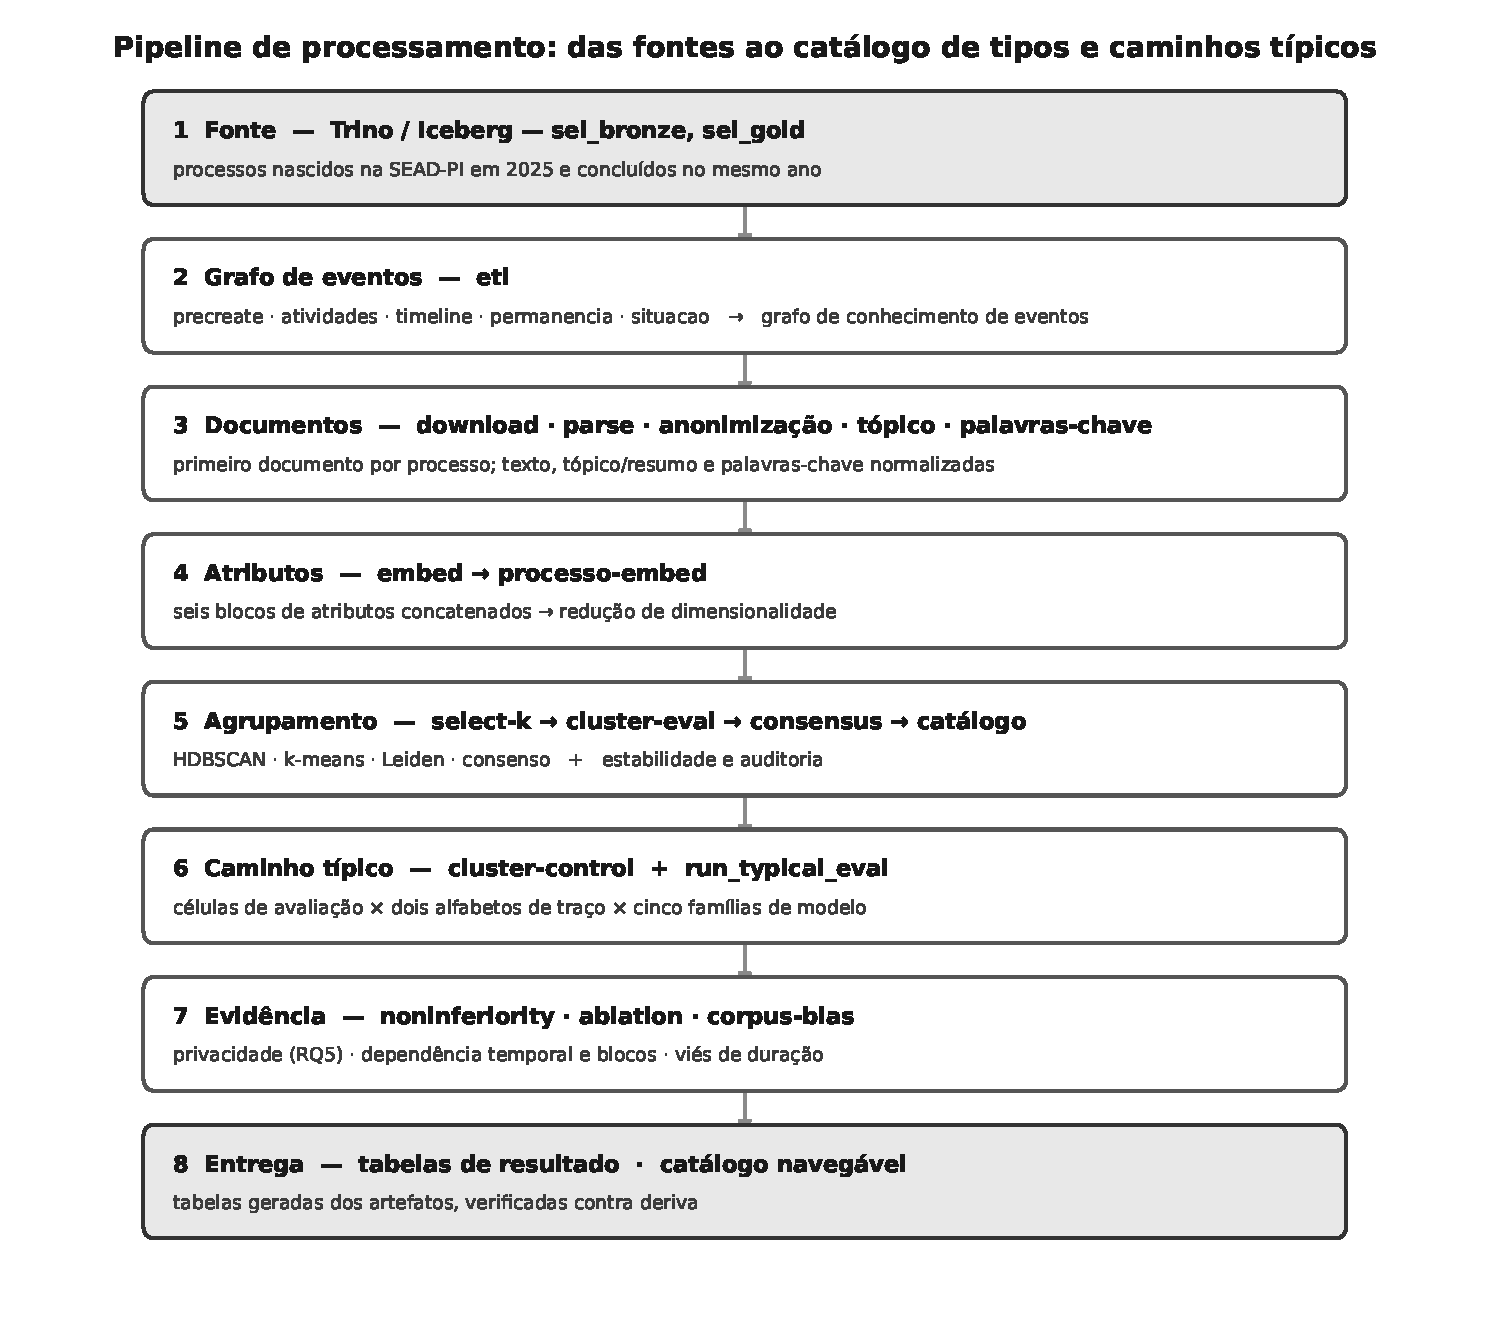
\includegraphics[width=\textwidth]{pipeline-macro.pdf}
\par\vspace{2pt}\footnotesize\raggedright O fluxo ilustra a sequência de extração, anonimização, vetorização, agrupamento e geração de caminhos típicos.
\end{figure}

\subsection{Caracterização da Pesquisa e Posicionalidade}\label{sec:caracterizacao}

Trata-se de uma pesquisa aplicada e quantitativa, caracterizada como estudo de caso único na SEAD-PI, com dados do ano de 2025. Conforme declarado na introdução, o vínculo funcional do autor com a secretaria exigiu a adoção de salvaguardas rigorosas (anonimização automatizada, processamento local e validação contra \emph{baselines} cegas) para evitar vieses e garantir o alinhamento com a autorização institucional de tratamento de dados \cite{seadpi2026termo}.

Neste texto, adota-se a seguinte convenção: \textbf{processo administrativo} refere-se ao caso individual analisado; \textbf{tipo de processo} é o agrupamento resultante (o \emph{cluster}); \textbf{traço} é a sequência de eventos de um processo; e \textbf{ação} é a tipologia do andamento registrado pelo sistema.

\subsection{Cenário, Corpus e Recorte Analítico}\label{sec:corpus}

O SEI não restringe as trajetórias dos processos administrativos. Embora as ações sigam ordem cronológica, um processo pode tramitar simultaneamente em múltiplas unidades. Para viabilizar a modelagem sequencial, este comportamento concorrente foi linearizado adotando-se a ordem cronológica estrita dos carimbos de tempo dos eventos.

Os dados foram extraídos do \emph{data lakehouse} da SEAD-PI (tabelas Iceberg via Trino). O recorte incluiu exclusivamente processos iniciados e concluídos na Secretaria no ano civil de 2025 que possuíam documento inicial legível. De 12.621 processos gerados, 5.445 foram carregados e \textbf{5.243} atenderam a todos os critérios e compõem o corpus da análise.

\subsubsection{Viés de Censura à Direita}\label{sec:vies}
Exigir a conclusão dentro do mesmo ano civil trunca a amostra, penalizando processos longos iniciados nos últimos meses do ano. Estimou-se um déficit de 18,2\% na população concluída, concentrado em trâmites prolongados. Consequentemente, o corpus não reflete durações médias globais de processamento, limitando inferências sobre eficiência temporal absoluta (Tabela~\ref{tab:corpus-bias}).

%% GENERATED by `pipeline run results` - do not edit by hand.
\begin{table}[htbp]
\centering
\caption{Censura à direita por mês de abertura.}\label{tab:corpus-bias}
\footnotesize
\begin{tabular}{lrrrrr}
\toprule
mês & observados & dias disponíveis & vida mediana & vida máxima & excl.\ estimada \\
\midrule
2025-01 & 474 & 365 & 21 & 343 & 0,0\% \\
2025-02 & 619 & 334 & 14 & 290 & 0,2\% \\
2025-03 & 478 & 306 & 17 & 284 & 0,8\% \\
2025-04 & 470 & 275 & 25 & 244 & 2,1\% \\
2025-05 & 415 & 245 & 24 & 225 & 5,1\% \\
2025-06 & 621 & 214 & 18 & 204 & 21,7\% \\
2025-07 & 653 & 184 & 12 & 166 & 24,1\% \\
2025-08 & 398 & 153 & 18 & 129 & 26,2\% \\
2025-09 & 539 & 122 & 10 & 105 & 29,3\% \\
2025-10 & 381 & 92 & 10 & 75 & 31,9\% \\
2025-11 & 268 & 61 & 5 & 42 & 35,9\% \\
2025-12 & 129 & 31 & 5 & 29 & 44,5\% \\
\bottomrule
\end{tabular}
\par\vspace{2pt}\footnotesize\raggedright Observados 5.445; verdadeiro estimado 6.658; ausentes estimados \textbf{1.213} (18,2\%). Limite inferior: o próprio mês de referência está truncado.
\end{table}


\subsection{Modelagem: Grafo de Conhecimento de Eventos}\label{sec:ekg}

Os \emph{logs} transacionais foram estruturados em um Grafo de Conhecimento de Eventos \cite{vanderaalst2016processmining, esser2021ekg}. A construção ocorreu em três etapas:
1. \textbf{Ingestão de Dimensões:} Criação de nós para unidades, usuários e tipos de procedimento.
2. \textbf{Anexação de Atividades:} Vinculação de cada atividade ao processo, unidade, usuário, ação e documento.
3. \textbf{Encadeamento Sequencial:} Conexão temporal das atividades do mesmo processo via relações de precedência direta.

A partir do grafo, derivaram-se as métricas de tempo de posse e retrabalho. Os traços gerados foram congelados em disco para isolar as fases de agrupamento e avaliação do banco de dados transacional.

\subsection{Processamento do Documento Inicial e Anonimização}\label{sec:documento}

Por exigência contratual da autorização de pesquisa \cite{seadpi2026termo}, a anonimização de dados pessoais antecedeu qualquer vetorização. O documento inicial foi convertido para texto plano (via extração nativa ou visão computacional local). Em seguida, aplicou-se uma dupla camada de detecção e supressão:
* \textbf{Mecanismos baseados em regras:} Validação de CPFs, CNPJs, e-mails e matrículas funcionais.
* \textbf{Reconhecimento de Entidades Nomeadas (NER):} Aplicação de um modelo neural de esquema aberto \cite{zaratiana2025gliner2} para substituir nomes próprios e informações sensíveis por marcadores consistentes (\emph{tokens} consistentes baseados no \emph{hash} da entidade, preservando a correferência).

A partir do texto limpo, um modelo de linguagem de pesos abertos gerou, para cada processo, um \textbf{tópico} e um \textbf{resumo} de uma frase, atuando como um filtro de ruído semântico. Além disso, extraiu-se um vocabulário controlado de palavras-chave através da unificação de n-gramas com similaridade de Dice $\geq 0,9$.

Para conformidade jurídica, toda inferência de rede neural foi executada no \emph{cluster} de alto desempenho local (Mandu, GPUs NVIDIA) do Governo do Estado do Piauí, sem chamadas a APIs externas.

\subsection{Vetorização e Agrupamento}\label{sec:atributos}

Cada processo administrativo foi representado pela concatenação de seis blocos de atributos, posteriormente reduzidos a 50 dimensões via UMAP \cite{mcinnes2018umap} (distância de cosseno):
1. \emph{Embeddings} do documento inicial (1.024 dimensões, via BGE-M3 \cite{chen2024bgem3}).
2. \emph{Embeddings} do tópico e resumo gerados (1.024 dimensões).
3. TF-IDF das unidades organizacionais visitadas (500 dimensões).
4. TF-IDF das transições entre unidades (1.000 dimensões).
5. Histograma de tipos de ações (48 dimensões).
6. TF-IDF das palavras-chave do documento (517 dimensões).

O agrupamento operou sobre esse espaço vetorial utilizando três famílias algorítmicas, varrendo hiperparâmetros para garantir robustez aos métodos: \textbf{HDBSCAN} (densidade) \cite{mcinnes2017hdbscan}, \textbf{K-means} (centroides) e \textbf{Leiden} (modularidade em grafos) \cite{traag2019leiden}. Essa grade gerou 14 configurações de clusterização (sete por braço: anonimizado vs. bruto). Processos não atribuídos pelo modelo de densidade (ruído) foram realocados ao centroide mais próximo para equalizar a população de avaliação entre os algoritmos.

\subsection{Alfabetos de Traço e Caminhos Típicos}\label{sec:caminhos}

A avaliação ocorreu separadamente sob três abstrações de alfabeto (Figura~\ref{fig:alfabetos}):

\begin{figure}[htbp]
\centering
% 1. O caption agora atua apenas como TÍTULO (conciso e direto)
\caption{Um mesmo processo administrativo renderizado nos três alfabetos de traço.}
\label{fig:alfabetos}

\fbox{\begin{minipage}{0.93\textwidth}
\vspace{2pt}
\raggedright\footnotesize
\textbf{Alfabeto de ação por unidade} --- excerto dos dezoito estados:

\vspace{2pt}
\texttt{GERACAO-PROCEDIMENTO@UNIDADE-A} · \texttt{GERACAO-DOCUMENTO@UNIDADE-A} ·
\texttt{ASSINATURA-DOCUMENTO@UNIDADE-A} · \texttt{CONCLUSAO-AUTOMATICA@UNIDADE-A} ·
\texttt{PROCESSO-REMETIDO@UNIDADE-B} · \texttt{PROCESSO-RECEBIDO@UNIDADE-B} ·
\texttt{GERACAO-DOCUMENTO@UNIDADE-B} · \ldots ·
\texttt{CONCLUSAO-PROCESSO@UNIDADE-A}

\vspace{6pt}
\textbf{Alfabeto de roteamento} --- os mesmos dezoito estados, colapsados em três:

\vspace{2pt}
\texttt{UNIDADE-A} $\rightarrow$ \texttt{UNIDADE-B} $\rightarrow$ \texttt{UNIDADE-A}

\vspace{6pt}
\textbf{Alfabeto de procedimento} --- os mesmos dezoito estados, abstraídos do organograma:

\vspace{2pt}
\texttt{GERACAO-PROCEDIMENTO} $\rightarrow$ \texttt{GERACAO-DOCUMENTO} $\rightarrow$
\texttt{ASSINATURA-DOCUMENTO} $\rightarrow$ \texttt{PROCESSO-REMETIDO} $\rightarrow$
\texttt{PROCESSO-RECEBIDO} $\rightarrow$ \texttt{GERACAO-DOCUMENTO} $\rightarrow$ \ldots
$\rightarrow$ \texttt{CONCLUSAO-PROCESSO}
\vspace{3pt}
\end{minipage}}

% 2. A legenda/nota explicativa vai para baixo, agrupando toda a explicação
\vspace{4pt}
\begin{minipage}{0.93\textwidth}
\footnotesize\justifying
\textbf{Nota:} O alfabeto de ação por unidade conserva o que se fez e onde; o de roteamento conserva apenas por onde o processo passou; o de procedimento conserva apenas o que se fez. Os dois últimos colapsam repetições consecutivas, avaliando populações distintas. A diferença central é a granularidade da representação: \texttt{ação@unidade} preserva localização, \texttt{roteamento} preserva trajetória e \texttt{procedimento} preserva ação.
\end{minipage}
\end{figure}

* \textbf{Ação por Unidade:} Estado completo não projetado (\emph{ação@unidade}).
* \textbf{Roteamento:} Sequência apenas das unidades organizacionais (foco organizacional).
* \textbf{Procedimento:} Sequência apenas das ações executadas (foco procedimental).

Para cada \emph{cluster} contendo ao menos 30 processos, ajustaram-se seis geradores sequenciais para predizer o próximo evento e compor o "caminho típico": Markov (3ª ordem), Grafo de Precedência Direta (DFG), GRU \cite{cho2014gru}, LSTM \cite{hochreiter1997lstm}, Transformer \cite{vaswani2017attention} e Redes Convolucionais em Grafos (GNN) \cite{kipf2017gcn}. Os hiperparâmetros das redes neurais foram fixados para evitar que a comparação capturasse apenas esforço de sintonia.

A geração foi submetida a uma decodificação restrita via máquina de estados, impedindo predições que violassem as regras sistêmicas de movimentação do SEI (ex: concluir um processo nunca recebido).

\subsection{Protocolo de Avaliação e Variáveis de Controle}\label{sec:protocolo}

Os processos foram particionados em 70\% (treino) e 30\% (teste). A métrica primária foi a \textbf{acurácia de próximo passo}, complementada por validações de sustentação de caminho (cobertura e suporte de transições observadas na realidade). 

Para isolar a qualidade da modelagem estrutural do mero "dividendo de partição" (facilidade inerente de prever vocabulários menores em grupos menores), utilizaram-se três linhas de base:
1. \textbf{Sucessor Intragrupo:} Predição pela frequência máxima de transição.
2. \textbf{Modelo Global:} Um único modelo (Markov 3ª ordem) treinado sobre todo o corpus.
3. \textbf{Partição Embaralhada:} Troca aleatória de rótulos dos processos, preservando tamanho e quantidade dos clusters, mas destruindo a pertinência semântica. 

O estimando principal ($\Delta^*$) consistiu na diferença de acurácia agregada ponderada entre a partição real proposta e a sua equivalente embaralhada. Uma partição cujo $\Delta^*$ não seja significativamente positivo foi considerada como não portadora de sinal latente útil.